\documentclass[11pt, a4paper ]{article}

\usepackage[utf8]{inputenc}
\usepackage[T1]{fontenc}
\usepackage[top=2.5cm, bottom=2.5cm, left=2.5cm, right=2.5cm]{geometry}
\usepackage[francais]{babel}
\usepackage{wrapfig}
\usepackage{graphicx}
\usepackage{makeidx}
\usepackage{url}
\usepackage{tabularx}
\usepackage{setspace}
\makeindex
%\usepackage{fontspec}
%\setmainfont{Arial}

\title{Mémoire Titre qui en jette grave}
\author{Julien Prugne 108287}
\date{Avril 2014 à Octobre 2014}

% new page for every section
\let\stdsection\section
\renewcommand\section{\newpage\stdsection}

\begin{document}
\begin{spacing}{1.5}

	\maketitle
	\tableofcontents

	% TODO: à la toute fin

	\section{Introduction} %3 pages

	% TODO: avant intro et conclusion
	% récolter assez d'info
	%\chapter{présentation entreprise et mise en context : titre personalisé} % 25 pages


	\section{Présentation de l'entreprise: titre personnalisé} % 15 pages trouver un meilleur titre

			%intro de partie
DOM Element Inc. est une startup Montrealaise.

Une startup\cite{theseStartup} est une jeune entreprise. C'est une structure ayant pour but de déffricher un nouveau pan de l'economie. Il s'agit d'entreprise généralement incarné par leur(s) créateur(s) et fondant son modéles économique sur l'innovation. Cette capacité innovation est l'adn des startups.

Dans un premier temps l'entreprise en elle même n'est qu'une structure légale offrant une interface avec des stuctures ayant la capacité de financer l'essort du projet. En effet, les plan d'affaires de ces entreprises prévois généralement des pertes sur les premiers temps de son dévellopement voir pour l'intégralité de son existence. Cela peut sembler incohérent à premier abord mais un écosystéme c'est créer autour des startups. Riche particuliers\footnote{Bussiness Angel}, des groupe financier gérant un fond privé\footnote{venture capital}, concours entrepreunarial créer un flux entrant de capitaux dans cette économie. Ces derniers ont généralement pour objectif de rentabiliser leurs investissements lors de la vente ou de la capitalisation boursiére de la startup. Les montants en jeux sont considérable, les investissements ou les ventes de telle sociétées ce chiffre en dizaine, centaine de millier de dollars certain cas allant jusqu'à plusieurs milliards de dollars.

Les perspectives de ces marchés semblent extrémement interessante mais il faut pondérer ces assertions par le taux d'échec impressionnant des start-up. En effet, au bout de 4 ans seul cinquante pourcent des startup ssemble encore en activité le tout chute drastiquement au bout de dix ans seul vingt-neux pourcent d'entre elles sont encore en activité.
Beaucoup de chiffre pourrais être cité de nombreuse sources mais vue que cette économie est encore sauvage et peux controllé ou controllable mais les statistique semble s'accorder sur une tendance générale: Le taux d'échecs des startup est colossale mais les réussites sont spéctaculaire.

La majorité  arretera par manque de moyen financier empéchant de mener le projet à maturité,  puis une petite portion sera acheter par de gros groupe\footnote{ skype par microsoft pour 8,5 milliards de dollars, instagram par facebook pour 1 milliard de dollar,... } et enfin une infime petite partie deviendront de large entreprise\footnote{exemple: facebook, twitter, Google,...} aprés capitalisation.

\begin{center}
	\begin{tabular}{l*{1}{c}}
		Années  & Taux d'échec\\
		\hline
		1 & 25\% \\
		4 & 50\% \\
		7 & 63\% \\
		10 & 71\% \\
	\end{tabular}\cite{statEchecStartup}
\end{center}

Attention toute les jeunes entreprises ne sont pas des startups. Une startup est caractérisé par sa capacité à générer de la croissance rapidement. Le taux de croissance hebdomadaire de croissance est l'indicateurs le plus révélateur de la bonne santé d'une startup.

\begin{quote}
	[...]

	Commençons par faire une ditinction qui est souvent ignoré: tout les compagnie financé ne sont pas des startups. Des millions de compagnie sont créer chaque années aux États Unis. Seul une petite fraction de ces entreprises sont des startups. La pluspart sont des services commerciaux - restaurants, coiffeurs, plombier, etc. Ce ne sont pas des startup sauf dans quelques cas particuliers. Un salon de coiffure n'est pas précue pour une croissance exponentiel. Tandis qu'un moteur de recherche l'est.

	[...]


	\caption{Paul Graham, \emph{Startup = Growth\cite{startupGrowth}}}
\end{quote}

Une startup est donc avant tout un projet soutenue par une équipe passionné et persuader de la pertinence et de la capacité à générer de la croissance de leurs solutions. Pour happybox, c'est de rendre la création web abstraite de toute contraintes techniques.

		% présentation générale HappyboxCMS = intro plan d'affaire
		%	historique à étoffer
		\subsection{L'équipe} %2 pages max
DOM Element étant une trés petite structure composé principalement de ses deux co-fondateurs: Danny Coulombe et Guillaume Lagacé, de deux actionnaires minoritaire chargé de la communication: Brendan Shera-shriar et Brendan Tully-Walsh et de un ou deux stagiaire selon l'époque: François Lacroix-Durant et moi même.

\begin{center}
	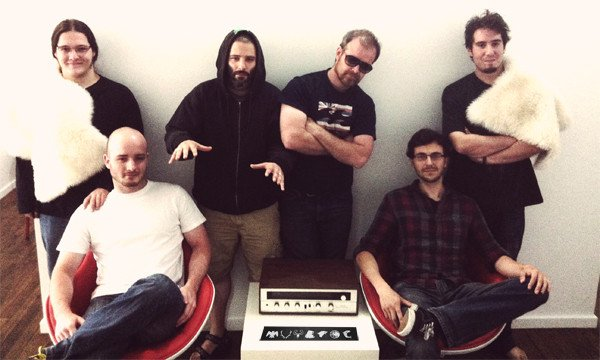
\includegraphics[width=\textwidth]{images/team/team.jpg}

	 De gauche à droite: François Lacroix-Durant, Danny Coulombe, Brendan Sera-Shriar, Brendan Tully Walsh, Guillaume Lagacé and Julien Prugne.
\end{center}

\paragraph{}
	Guillaume Lagacé à le rôle de \emph{CEO}, Chief Executif Officer ou Président Directeur Générale en français, Il à pour responsabilité de mettre en place la structure globale de l'entreprise.
	Ses tâches inclus:

		\begin{itemize}
			\item
				Relations avec les financiers
			\item
				Définitions de la stratégie d'entreprise.
			\item
				Coordination de l'équipe
			\item
				Entretiens les relations d'affaires
		\end{itemize}

\paragraph{}
	Danny Coulombe est le \emph{CTO}, Chief Technolgy Officer ou Directeure de la Technologie en français. Il est le dévellopeur principale d'Happybox CMS. Il est responsable des orientation technologique et de la gouvernance du dévelopement du produit.



	Ces tâche inclus:

		\begin{itemize}

			\item
				Dévelopement \emph{Full Stack\footnote{Expression en vogue désignant un dévelopeur web alliant à la fois de compétence de dévellopement front-end et bakend ainsi que des compétences en administration systémes. Il s'agit d'un profil complet capable de créer, déployer et maintenir une application web dans sa totalité.}}
			\item
				Design interface utilisateur
			\item
				Optimisation d'experience utilisateur
			\item
				Prototypage

		\end{itemize}



\paragraph{} %brendans
	\emph{The Brendans} est une agence de communication digitale anglophone Montrealaise. Ses deux membres fondateurs, Brendan Shera-Shriar et Brendan Tully-Walsh, sont actuellement actionnaire à hauteur de 2\%. Ils ont pour mission avec leur équipe de promouvoir Happybox CMS sur les réseaux sociaux, de créer et d'entretenir l'image du produit.
	C'est un élément fondamentale de l'accès au web. Seul les compagnies ayant une bonne visibilité auprès de leur cible et entretenant ded rapportd avec leurd clients semblent émergé.

		\subsection{Historique DOM Element Inc.}
%%%%%%%%%% TODO: INTEGRER LE RESEAUX ET LES CONCOURS ICITTE %%%%%%%%%%%%%%%%%
% Avril 2013 Fondation Montréal Inc. (12 000)
% Juin 2013 Jeunes Promoteurs (18 000)
% Février 2014 SDEVM (10 000)

\paragraph{}
\emph{Happybox CMS}, a vu le jour en Octobre 2012, lorsque Guillaume Lagacé et Danny Coulombe, fondateurs de l'agence digitale \emph{WebRight\footnote{\url{http://webright.ca/fr}}} décident d'élaborer un moteur de création web alliant simplicité d'utilisation, téchnologie de pointe et créativité.

\paragraph{}
Pour arriver à leurs fins, ils enregistrent la société \emph{DOM Element Incorporated} le 23 Octobre 2012 auprés du registraire des entreprises du Quebec via la société \emph{Dufourd, Dion Avocats}. Les droits du produit Happybox CMS sont cédés à \emph{DOM Element Inc}, Danny et Guillaume se partagent alors la compagnie en deux parts égales, leur conférant un pouvoir décisionel commun et équivalent au sein de l'entreprise.

\paragraph{}
Durant les deux mois suivants, les efforts s'orientent sur le dévelopement du projet \emph{Happybox CMS}.
En décembre 2013, l'équipe rencontre Brendan Shera-Shriar et Brendan Tully-Walsh, co-fondateurs de l'agence de communication digitale \emph{The Brendans} qui deviendront, le 15 mai 2013 des actionnaires et membres éxecutifs de DOM Element Incorporated en échange de leur expertise en terme de communication et d'acquisition de clientèle.


\paragraph{}
Ce même mois de mai 2013, Happybox CMS, nom de produit approuvé plus tôt en fevrier, est sélectionné pour faire partie de la \emph{cohorte de la fondation Montreal Inc.} et recevra une bourse de \$12000. Bourse qui sera uilisée pour le financement du dévelopement et de la communication autour du produit.

%%%%%%%%%%%%%%%%%%%%%%%%%%%%%%%%%%%%%%%
%%%%%% PARLER DES LOCAUX  + choix model freemium %%%%%%%
%%%%%%%%%%%%%%%%%%%%%%%%%%%%%%%%%%%%%%%

\paragraph{}
En juin 2013, François Lacroix-Durant et moi-même intégrons les rangs de DOM Element Inc., respectivement en tant qu'intégrateur web et administrateur systémes. à la même période happybox reçoit une bourse \$18,000 grâce au programme \emph{Jeunes Entrepreneurs} organisé par la société de dévelopement économique de Ville-Marie.

\paragraph{} %%%% raconter l'été 2013
Durant l'été 2013, nous nous installons dans loft partagé avec les Brendans situé dans le vieux port de Montreal. Nous avons, François, Guillaume, Danny et moi même passé l'été à déveloper le produits, les infrastrcutures nécessaire pour acceuillir Happybox CMS et modéles freemium actuellement en vigueur sur Happybox CMS.


\paragraph{}
À l'automne 2013, le service en ligne Happybox CMS ouvre ses portes pour une phase d'alpha privé comptant déjà une centaine d'utilisateurs. Principalement des dévelopeurs, des agences de Marketing Montréalaise ainsi que l'entreprise Maaco\footnote{Maaco est une des plus grande chaîne de peinture et de réparation de véhicules d'Amérique du nord.}.

\paragraph{}
Le 19 Novembre 2013, Happybox CMS se classe second au grand concours entrepreunarial \emph{Prix Montreal Inc}..
%%%%%% TODO: manquant décembre 2013 à maintenant %%%%%%%

\paragraph{}
En fevrier 2014, Dom element reçoit une nouvelle bourses de \$10,000 de la part de la Société de dévelopement économique de Ville-Marie.
%%%%%% FIN                                       %%%%%%%

			\subsection{Plan d'affaire: le modéle freemium} % 11 pages
% Là faut charger! cible tout du long

\paragraph{}
% intro model freemium
Le \emph{modéle freemium\index{freemium!modéle}} est un type de plan d'affaire. Le mot \emph{freemium} est la contraction de deux termes anglophones : \emph{free} et \emph{premium}. Ce modéle économique ce voue à proposer un produit ou un service gratuitement à la majorité de ses utilisateurs afin que tous puisse accéder librement au produit. En plus de cette offre gratuite, il est proposé à l'utilisateur une offre dite premium qui , elle, est payante et transforme une partie des utilisateurs en client générateur de revenue. La minorité des utilisateurs payant le service premium financeront la plateforme pour l'intégralité de ses utilisateurs.


% presentation détaillé
\paragraph{} % offre gratuite
L'offre gratuite ne peut pas et ne dois pas être une version d'essaie inutilisable sans recourir au service premium. Ce dois être un produit répondant à un besoin de l'utilisateur ou lui offrant un produit ou un service dont il aurait envie. Cette base d'utilisateurs gratuit est vitale au fonctionnement de cette stratégie d'affaire.

\subparagraph{} % exemple offre gratuite skype + farm ville
L'exemple le plus frappant est surement Skype, ce dernier propose un service de voix et de vidéo sur internet entiérement gratuit à ses urilisateurs. La majorité des utilisateurs ne paieront jamais pour utiliser un service le permettant de faire la visionconférence internationale gratuitement.

Un autre exemple populaire pourrait être les jeux de gestion sur facebook type \emph{farmville} porposant gratuitement des jeux complet, avec des mécaniques basé sur l'interaction sociale avec le réseaux du(de la) joueur(joueuse\footnote{La cible de prédilection de ces compagnies n'est pas la même que les autres compagnie de jeux vidéo car ces derniers ont du temps mais peu voir pas d'argent ni de carte de crédit, ils constitueront la masse des joueurs offrant la visibilité nécessaire au jeux. Le véritable marché cible de situe chez les ménagères d'âges moyen, femme au foyer qui semblent être les véritables payeuses des jeux sociaux. }) rendant le produit addictif pour ses utilisateurs.

\paragraph{} % offre payante
Il est évident que seul une offre gratuite ne peut suffire à garantir les revenues nécessaire au fonctionnement de l'entreprise. C'est la qu'interviens l'offre premium. C'est un complement à l'offre gratuite une amélioration significatif de l'experience utilisateur. Cette offre surclassé dois permettre de financer l'offre gratuite ou compenser dans un premier temps au maximum les cout de l'offre gratuite.
\subparagraph{}
L'offre premium peux porter sur différents type service mais dois toujours être en adéquation avec l'offre gratuite, de fait la définition de l'offre premium étant intimement lié au produit il est impossible de définir un modéle unique et applicable à tout type d'affaire. On remarque tout de même que de grande tendance semble ce dessiner et cela viens de la concurrence importante sur les marché porteurs de freemium ainsi beaucoup semble adopter la même ligne d'affaire et offir des services similaires du moment qu'il propose des offres similaire. La copie des plan d'affaire de société en pleine expansion est une stratégie vieille comme le monde.

\subparagraph{} % exmple skype et farmville

On ne compte plus le nombre de jeux gratuits sur facebook offrant des achats \emph{in app} ne coupant l'experience de jeux et permettant d'accélerer la progression des joueurs évitant ainsi d'avoir à subir l'arduité de l'experience de jeux optimisé pour la conversion des utilisateurs. L'achat sera donc le plus souvent impulsif pour gagner du temps de jeux afin de dépasser ses \emph{amis facebook} ou tout simplement de pouvoir continuer à jouer car dans ce genre d'application la tendance semble être à la limitations du nombre d'action effectuable par heure avec une possibilité de paiement pour éviter d'attendre\footnote{Il s'agit de coupe file numérique.}. Au moment ou ces lignes sont écrite \emph{Farmville 2 dévellopé par Zynga} compte dix millions d'utilisateurs mensuel seul 3\% de ces utilisateurs paieront une offre premium.


La cible de ces produits sont des amateurs de jeux néophyte en terme de pratique vidéoludique qui ne ce rendront pas compte que le rapport amusement/cout est un des plus mauvais sur le marché.

\subsubparagraph{}
Les applications d'écoute de musique\footnote{Spotify, Deezer, Groove Shark, Google Music, ...} propose généralement une offre gratuite incluant publicité durant les temps d'attente, des limitations sur le nombres de morceaux écoutable ainsi que le nombre d'écoute d'un même morceaux.
Le paiement d'un abonnement supprimera publicité et limitation ainsi que l'ajout de de fonctionnalité type synchronisation des fichiers sur un appareil afin d'offrir un accés hors ligne. Plusieurs type d'offre payante pourront ainsi être proposé.

%%% offre premium spotify %%%

\paragraph{} %validité et limite du model
% citation freemium.org => equations
	\subparagraph{} % comment c'est possible de faire payer 5% de ses clients?
Le concept de freemium peux sembler frauduleux à premiére vue. En effet, un modéle économique basé sur la distribution gratuite de son produit semble d'emblé voué à l'échec. Il est difficile d'imaginer un boulanger offrant gratuitement ses croissants en espérant financer son affaire via la vente d'offre surclassé comme un croissant avec de la confiture, un sac de transport en tissu issus du commerce équitable et un sourire de la caissière. Une telle pratique économique ne peut être perreine. De maniére générale toute offre implicant la disparition du bien\footnote{Les fameux croissants ou tout autre bien de consommation.} ou du service\footnote{Coiffeur, avocat, medecin, ...} après utilisation ne semble pas adapté au modéle freemium.
\subparagraph{}
Ce qui rend cette solution viable dans le cadre d'un produit digitale et le faible cout de duplication et de distribution du produit\footnote{Que ce soit un biens ou un service.}. Un logiciel traditionel, une fois dévellopé ne coute pas plus chére si il est éxécuté une fois ou 10 fois sur le poste d'un client. Il en va de même pour les biens culturels\footnote{Le groupe de musique \emph{Nine Inch Nails} à offert son album en mp3 téléchargeable gratuitement. Les support physique en édition de collection vendue plus chère qu'un disque conventionel, les produits dérivé et la vente de billets de concert constitue l'offre premium du groupe. La distribution et la duplication de fichiers musicaux étant nulle l'offre premium paiera les musiciens et rentabilisera les coûts de production.}, par exemple un livre une fois écrit et convertis dans un format numérique à le même cout de production peut importe le nombre de ses lecteurs. La magie de ce paradigme viens du fait que copier un fichier est une opération logiciel simple qui n'altére ni ne supprime le fichier originale quelqu'en soit le nombre de copie effectué. Le cout de production d'une copie du produits s'approche alors de zéro.
\subparagraph{}
Il ne faut surtout pas considérer un utilisateur gratuit comme une perte car un consommateur ne payant pas le produit n'est pas un client, c'est un moyen. Au même titre que l'achat d'encars publicitaire, de mot clé dans les moteurs de recherche ou de publication mise en avant sur les réseaux sociaux pour faire la promotion du produit.
En proposant un service ayant, aux yeux de l' utilisateur, une réel valeur ajouté qui le pousserai à utiliser réguiliérement on crée une \emph{relation d'approbation} qui à une valeurs bien supérieur à la publicité.
En effet, si demain la boucherie de mon quartier adopte le modéle freemium en offrant gratuitement ses produits à tout les clients potentiels et offrant un service de charcuterie premium.
Il est plus que probable que je diffuse l'information auprés de mon réseaux qui le diffusera lui aussi à son réseaux et ainsi de suite jusqu'à atteindre la limite du marché, dans ce cas précis un cout de déplacement supérieur au gain apporter par le produit gratuits.
Dépenser \$200 d'essence pour obtenir un produit gratuit d'une valeur de quelque dizaine de dollars n'est pas judicieux. Il est toujours envisageable de compter sur une clientéle stupide mais mon expérience du jeux de go m'a appris qu'établir une stratégie basé sur les erreurs potentiels de son adversaire n'est que rarement voir jamais payant.
Considérer ses futurs clients\footnote{aka utilisateurs gratuits ou leurs réseaux} comme moutons à tondre ne peut être une stratégie payante à long terme même si à court termes de telles méthodes peuvent apporter des recettes.
\subparagraph{}
Attention les pratiques trop agressive auprés de l'utilisateurs l'entrainera peut être à court termes à acheter et augmenter les revenues de la compagnie mais, trés vite, l'utilisateur ce lassera plus vite et quittera la plateforme réduisant à néant toute stratégie de rétention d'utilisateurs à long terme. Depuis sa capitalisation boursiére la compagnie Zynga\footnote{Zynga, société créatrice de Farmville ainsi que 67 autres jeux gratuits sur le réseaux sociale facebook, à fait sont offre public initial, IPO, le 26 décembre 2011 évaluant l'entreprise aprés son entré en bourse à environ 7 milliards de dollars.\cite{ipoZynga}} tente d'achever sa profitabilité et adopte une stratégie de plus en plus agressive auprès de sa communautée de joueurs pour augmenter leurs consommation et les revenues de la société. Ces campagnes on eu pour effet une chute drastique, -68.55\% entre le quatième trimestre 2012 et le troisième trimestre 2014 du nombre d'utilisateurs.
% source http://www.appmtr.com/facebook/app/321574327904696-farmville-2/

\begin{center}
	\begin{tabular}{|l*{1}|c|c|}
		Trimestre  & utilisateur actif mensuel & Variation\\
		\hline
		2012 T4 & 51,569,209 & 0 \\
		2013 T1 & 40,557,507 & - 21.35\% \\
		2013 T2 & 34,713,652 & - 14.41\% \\
		2013 T3 & 26,268,910 & - 24,32\% \\
		2013 T4 & 23,630,665 & - 10.04\% \\
		2014 T1 & 19,339,065 & - 18.16\% \\
		2014 T2 & 22,471,919 & + 16.20\% \\
		2014 T3 & 19,826,868 & - 11.77\% \\
	\end{tabular}\cite{appmtrFarmVille2}
	\label{Evolution du nombre d'utilisateur mensuel du jeux Farmville 2}
\end{center}

% Les restrictions sur les fonctionnalités (e.g. une version "lite" d’un logiciel) ;
% Les restrictions sur la quantité (e.g. un pack spécifique d’hébergement qui limite à 10 le nombre de base de données que l’on peut créer) ;
% Les restrictions sur le nombre de copie (e.g. un logiciel qui ne peut être installé que sur un unique ordinateur et non sur un réseau) ;
% Les restrictions sur les classes d’utilisateurs (e.g. un logiciel gratuit tant que l’utilisation est non commerciale) ;
% Les restrictions sur l’effort (e.g. un logiciel gratuit mais limité qui peut être débloqué gratuitement mais au prix de démarches laborieuses, qui peuvent être facilitées moyennant un paiement).
\subparagraph{}
Un modéle freemium, si il veux survivre à long terme dois être conçu et mise en place de maniére éthique\cite{ethicalF2P} en respectant les utilisateurs. Beaucoup d'offre freemium cherche à tirer un maximum de bénéfice, le plus rapidement possible, de ce qui semble être en ce moment un plan d'affaire extremement lucratif, ne cherchant pas la rétention à long termes des utilisateurs. Dans le cas des jeux gratuits contenant de la consommation en jeux, beaucoup fonctionne exactement de la même maniére. Parfois, il suffit de changer l'emballage pour donner l'impression de nouveauté suffisante à délier la bourse des plus impulsif.
\subparagraph{}
Il est donc fondamentale de connaitre exactement ses coûts de production et de distribution avant d'envisager un modéle tel que celui-ci. Pour cela, il faut savoir qu'il existe plusieurs types de coûts.
Les premiers sont les \emph{coûts fixe\index{Coûts fixe!définition}}\footnote{Exemple de coûts fixe: Loyer, Salaire des employées permanents, frais de justice, etc}\cite{defCoutFixeEtVar}, il ne varie pas en fonction du volume d'activité de l'entreprise.
À l'inverse, les \emph{coûts variables\index{Coûts variables!définition}\footnote{Exemple de coûts variables: Consommation éléctrique dasn une manufacture, salaire des employés temporaires, location d'instances sur Amazon Web Services pour répondre à la demande utilisateur.}\cite{defCoutFixeEtVar}}\ sont proportionnellement liés au volumes d'activité de l'entreprises, plus cette derniéres génère de l'activité, plus ses coûts variables vont augmenter.
Viens ensuite le tours des coûts d'opportunité\index{Coûts d'opportunité!définition}\footnote{Exemple de coûts d'opportunité: dépots de grantis à la création d'un compte en banque }\cite{defCoutOpp} qui sont un manque à gagner sur l'exploitation de capitale, c'est à dire que dans une situation donnée une somme d'argent à été bloqué ou investit, si ces actifs n'avait pas été bloqué il serait utilisé pour l'essort de l'entreprise. Un cout d'opportunité est donc la différence du résultat de l'action effectué minoré par le gain potentiel d'une autres utilisation de la ressource, c'est donc un coûts purement spéculatif.
Finalement, les \emph{coûts marginaux\footnote{Exemple de coûts marginaux: frais d'importation, }}\index{Coûts marginaux!définition}, définissent les frais necessaires à la production d'une commande suplémentaire. Il cherche à définir la rentabilité prévisionnelle d'une action donnée. Il est lui aussi purement spéculatif car c'est avant out un indicateurs stratégique.
\subparagraph{}
Les coût doivent être estimer de manières précise afin de pouvoir calculer ce que coût un utilisateurs gratuit. Une fois le coût réel d'un utilisateurs gratuit déterminé, il est nécessaire de connaitre le taux de conversion de ses utilisateurs gratuit en utilisateurs payant. Si l'on multiplie ensuite le nombre d'utilisateurs par le taux de conversion qui multiplie la contribution unitaire de chaque utilisateur on obtient une estimations de ses revenue\cite{equationFreemium}.

%%%% synthèse par les équation %%%%%
\begin{equation}\index{U!définition}
	U\ =\ Nombre\ d'utilisateur\ gratuit
\end{equation}


\begin{equation}\index{T!définition}
	T\ =\ Taux\ de\ conversion
\end{equation}


\begin{equation} \index{Cu!définition}
	Cu\ =\ Contribution\ unitaire\ moyenne\ par\ utilisateur payant
\end{equation}


\begin{equation}\index{Revenue!définition}
	U \times T \times Cu\ =\ Revenue
\end{equation}

Lorsque cet indicateurs est calculé il faut en calculer un second: les couts variables. C'est à dire une estimation du cout total des utilisateurs gratuit. Pour cela rien de plus simple multiplié le nombre de vos utilisateurs gratuit par le cout d'un utilisateurs. Ces utilisateurs ne sont pas des couts fixe car le montant exact de leurs utilisations dépendra du context de l'offre freemium.

%%%%%% synthese equations %%%%%%%
\begin{equation}\index{Cg!définition}
	Cg\ =\ cout\ d'un\ utilisateur\ gratuit
\end{equation}


\begin{equation}\index{Couts variables!calcule}
	U\ \times\ Cg\ =\ Couts\ variables
\end{equation}

Si en soustrayant aux revenues les coûts variables et que le résultats de l'opération est engendré aux coûts engendré par la création et la distribution du produit alors, théoriquement, le modéle est économiquement viable.

%%%%% synthese equation %%%%%%
\begin{equation}
	C\ =\ Coûts\ fixes\ +\ Couts\ Variables\ +\ Couts\ spéculatifs
\end{equation}
\begin{equation}
	(Revenue\ -\ Couts\ variables)\ <\ C
\end{equation}

% présentation du modéle freemium happybox
\paragraph{} % Happybox avec chiffres
Le choix du freemium pour Happybox CMS est le résultats de longues discussion avec la totalité de l'équipe lors de l'été 2013. De ces réunions nous avons établie pour chaque fonctionnalitée du produit les limites de l'offre gratuite et offert une solution de monétisation de l'offre premium\footnote{Voir en annexe le document récapitulatif rédigé en Aout 2013 par François Lacroix-Durant}.
Trois offres ont alors vue le jours au seins de l'application:

\begin{center}
	\begin{tabular}{|l|l|l|l|}
		Métrique & Personnel & Professionel & Agence \\
		\hline
		Domaine & sous domaine de happyboxcms.me & domaine personnalisé & domaine personnalisé \\
		Nombre de projet & 1 & 25 & illimité \\
		Bande passante & 5GB par mois & 50GB par mois & 100GB par mois \\
		Espace disque & 1 GB & 10 GB & 100 GB \\
		Style & basique & basique & avancé \\
		Analyse de traffique & basique & avancé & avancé \\
		Contenue Dynamique & non compris & non compris & oui \\
		Support & communautaire & via ticket & via ticket et téléphone  \\
		Prix & Gratuit & \$49.99/mois & \$100/mois\footnote{Ou négocié en fonction des services demandés.} \\

	\end{tabular}
\end{center}
\subparagraph{}
En applicants les équations vue dans les paragraphes précédents aves des chiffres prévisionnel basé sur une \emph{croissance\index{startup!croissance} de la masse des utilisateurs de 4\%\footnote{Croissance minimum hebodmadaire d'une startup afin d'attirer des capitaux issus du \emph{venture capitalisme}} selon Paul Graham fondateur de Y-Combinators. C'est aussi le taux de croissance prévitionnel définie dans le plan d'affaire de DOM Element Inc..} par semaine.
Spéculons sur un lancement discret en janvier 2014 avec cinquante utilisateurs gratuits trié sur le volet et un taux de conversions faible de 2\% aux vues du cout minimum par contribution unitaire actuel de \$49.99. Ces chiffres sont volontairement faible afin de voire si même avec des indicateurs ne permettant que difficilement d'atteindre les objectifs de rentabilités cela est possible. La profitabilité n'étant pas nécessairement un objectif pour une startup nous verrons pourquoi dans la section sur les mode de financement des startup.


%%% PRESENTATION

	\begin{tabular}{|l||c|c|c|}
		Temps & Utilisateurs gratuits & Utilisateurs payant & Cout utilisateurs\footnote{La méthodologie exact de calcule du cout par utilisateurs est présenté en détail dans la section .}\\ %%%% AJOUTER LE NUMERO DE SECTION
		\hline
		Janvier 2014 & 50 & 1 & \$0.52 \\
		Juin 2014 & 95 & 1.9 & \$0.48 \\
		Janvier 2015 & 291 & 5.82 & \$0.45 \\
		Juin 2015 & 649 & 12.98 & \$0.45 \\
		Janvier 2016 & 1,994 & 39.88 & \$0.44 \\
		Juin 2016 & 4,442 & 88.84 & \$0.44 \\
	\end{tabular}

\subparagraph{}
Il est possible de continuer d'appliquer les formules présenter dans la partie précédente afin de dégager une prévision théorique de revenue si le taux de croissance des utilisateurs reste stables durant les trois prochaines années en en Juin 2016 Happybox CMS devrait compter 4,442 utilisateurs dont 88.84 payant avec un achat unitaire de \$49.99 on obtiens un revenue de \$4,441.8 auquel il faut retrancher les coûts variables de \$1958.77 afin d'obtenir un résultat d'exploitation de positif de \$2483.03.

%%% PRESENTATION

	\begin{tabular}{| 1*{l} || c | c | c |}
		Temps & Cout Variable & Revenue & Resultat hors frais fixe\\
		\hline
		Janvier 2014 & \$26.26 & \$49.99 & + \$23.73\\
		Juin 2014 & \$46.06 & \$94.90 & + \$48.84\\
		Janvier 2015 & \$132.30 & \$291.35 & + \$159.05\\
		Juin 2015 & \$289.82 & \$649.22 & + \$359.4\\
		Janvier 2016 & \$881.63 & \$1,993.18 & + \$1111.55\\
		Juin 2016 & \$1958.77 & \$4,441.8 & + \$2483.03\\
	\end{tabular}



\subparagraph{}
Afin de clarifier ces projections voilà un graphique synthétisants les projections d'Happybox CMS en terme de croissance d'utilisateurs et de flux financiers, de ces derniers sont exclus les investissments, couts fixe, les couts d'opportunité ainsi que les coûts additionels. Pour plus de statistique rendez vous dans les annexes pour une foule de projection. Il est bien-sure evident qu'avec des indicateurs de base\footnote{Taux de croissance utilisateur, taux de conversion, contribution moyenne par utilisateurs payant} plus optimistes les résultats de ces projections seront meilleurs.

\begin{center}
	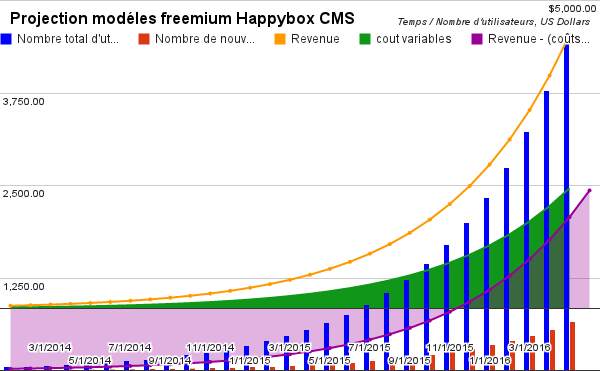
\includegraphics[width=\textwidth]{images/media/chartFreemiumHbCMS.png}
\end{center}

% \paragraph{}%limites

% Un certain nombres de limites sont déjà apparues tout au long de la présentation du modéle.

% - startup pas necessairement en quéte de revenue
% - croissance utilisateur = crédibilité face au investisseur = plus de roulement
% - clientele payante = bon point investissuer ça peu aller trés vite : Jeff Grammer partner Rho Canada startup breakfast montreal
% - source de financement des startup
% - croissance == danger pour les grosse entreprise en place qui ne veulent ==> rachat == objectif atteint
% - Modele freemium interessant pour startup evernote, skype, farmville
% - la croissance est ce qui permet à une startup d'atteindre sa maturité
% - User aquiring = absolue nécessité
% parrallel happybox

% = offre service ou produit gratuit
% - produit de qualité il faut des utilisateurs gratuit et le plus possible.
% - offre premium ajoutant des fonctionnalité payante
% - possible grace au coup quasi nulle de la duplication de bien digitale
% - mais pas que informatique, ex: musique distribution de mp3 gratuit offre premium: fichier de meilleur qualité, vente de support physique edition de collection, billet de concert, ...., nine inch nails album

% - On value un utilisateurs gratuit, c'est une source viral de communication, truc trop cool gratuit == truc géniale donc on en cause au pote qui en cause au pote. Effet de buzz rapide ==> plus d'utilisateur + de potentiel payeur
% - Il faut reellement fournir un service géniale dont les utilisateurs ont besoin! Sinon pas d'utilisateurs

% - taaux de conversion: utilisateur gratuit devenant utilisateur payant
% - Attention il est necessaire de connaitre exactement la valeur d'un utilisateur gratuit.

% - semble insensé mais




		\section{Un produit dans la jungle} % 10 pages
%%%%%%% Intro mise en context %%%%%%%%%%%%%%%%%%%%%
%Putain d'mise en contexte de mon cul!

%%%%%%%%%%%%%%%%%%%%%%%%%%%%%%%%%%%%%%%%%%%%%%%%%%%
			\subsection{Happybox CMS, une solution complète pour le web.}
		% présentation du produit avec screen et schéma technique (à traduire)

	% abstract
\paragraph{}
Happybox CMS est un logiciel en tant que service\index{SaaS!Happybox CMS}, c'est à dire qu'aucune installation n'est requise pour pouvoir l'utiliser. Il fonctionne sur un modèle client-serveur où le client est une page web dans votre navigateur communiquant avec un Service web, le serveur. Il faut le voir comme une feuille d'acétate qui se dépose sur un nom de domaine existant et permet instantanemment de créer un site web ou d'en éditer le contenu. 

% Dom Element Inc c'est une stratup donc orienter sur 1 seul et unique produit
%\subsubsection{Front end}
	% Présentation utilisateurs
	\paragraph{}
Happybox est avant toute chose un systéme de gestion de contenu\footnote{appellé aussi CMS, Content Management System}. Il s'agit d'un logiciel permettant la création et la mise à jour dynamique de site web.
C'est un CMS spécialisé dans la création de site web à une seul et unique page, appellé aussi \emph{page d'aterrissage} ou \emph{landing page} en anglais. Ce type de site web est généralement réserver au opération de promotions qu'elles soient personelles\footnote{Pages personnelle, présentation d'un projet, CV en ligne, loufoquerie, ...} ou corporative\footnote{Bon de réduction, présentation d'un produit, évenements, ...}. Il a pour objectif d'interesser les internautes afin de les informer ou de les guider vers un autre service.

%%%%%% TODO: causer SEO %%%%%%

%%%%%%%%%%%%%%%%%%%%%%%%%%%%%%

\paragraph{}
L'accés au service ce fait via une page Happybox présentant les différentes fonctionnalitées du logiciel. Cette page offre aussi un accés aux différents portails communautaires et à la création de compte. Ce site est une vitrine des possibilité offerte par le CMS. C'est le point d'accroche de la communication autour du produit.

%% SCREENSHOT ACCEUIL HAPPYBOX %%

\begin{center}
		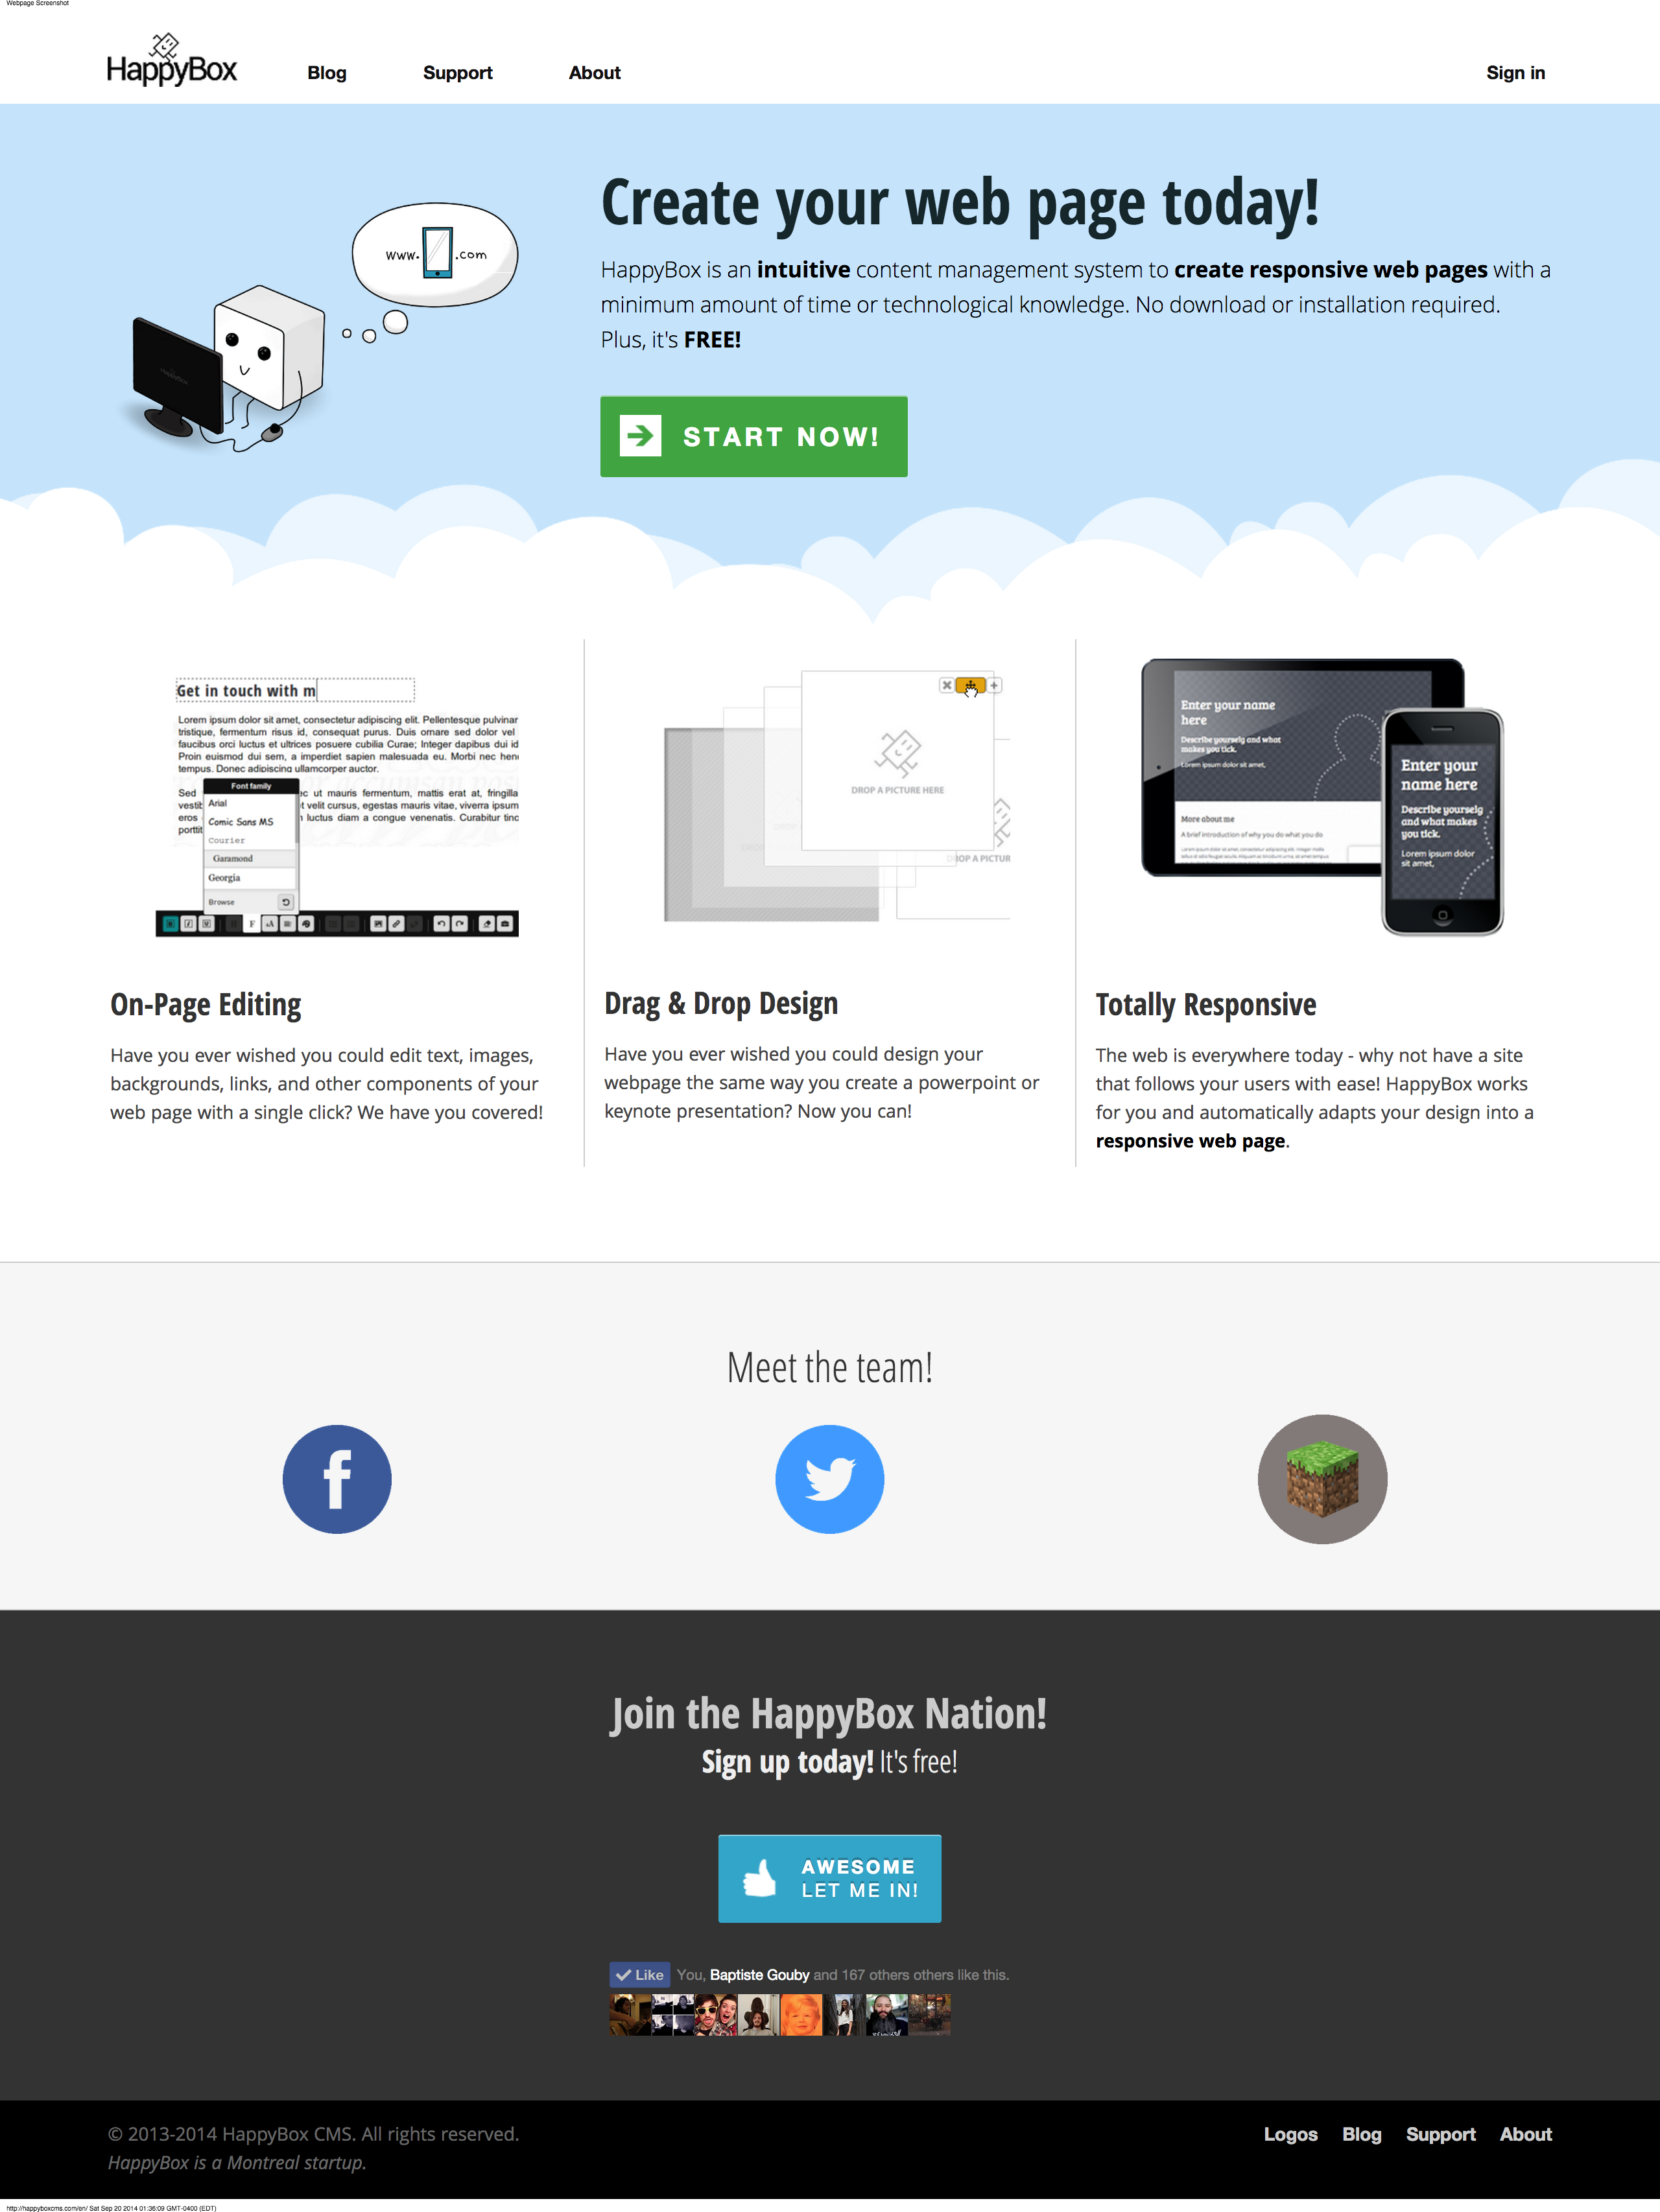
\includegraphics[width=\textwidth]{images/HBscreen/fullLanding.png}
		\caption{\url{http://happyboxcms.com} - Page d'aterrissage}
\end{center}

\paragraph{}
En effet Happybox CMS propose un éditeur de page intuitif, permettant en quelques cliques de définir un gabarit ou template de page. Le moteur ce base sur un systéme de grille, en effet les pages sont définies comme étant un ensemble de ligne ou section superposé les unes aux autres. Ces lignes peuvent être visibles ou non afin de créer des séparateurs sur la page\footnote{Section invisible laissant apparaitre le fond de la page.}. Dans ces sections, il est possible de définir des colonnes d'une largeur définis lors de la création du gabarit. Ces colonnes sont des conteneurs qui nous permettrons de stocker le contenue de la page par l'intermédiaire de \emph{widget\footnote{Élément textuel, titre, images, formulaire de contacts, liens, ...}}.

Chaque gabarit est complétement \emph{responsive\index{responsive!moteur de gabarit}}, c'est à dire qu'il s'adapte automatiquement à la résolution du navigateur client afin de garantir la meilleur expérience d'utilisation quelque que soit la plateforme utiliser pour consulter un site créer avec HappyboxCMS. La fonction de prévisualisation ainsi que les boutons en bas de l'éditeur permettent de tester son site pour chaque type d'appareil.


%% SCREENSHOT EDITEUR DE GABARIT%%
\begin{center}

		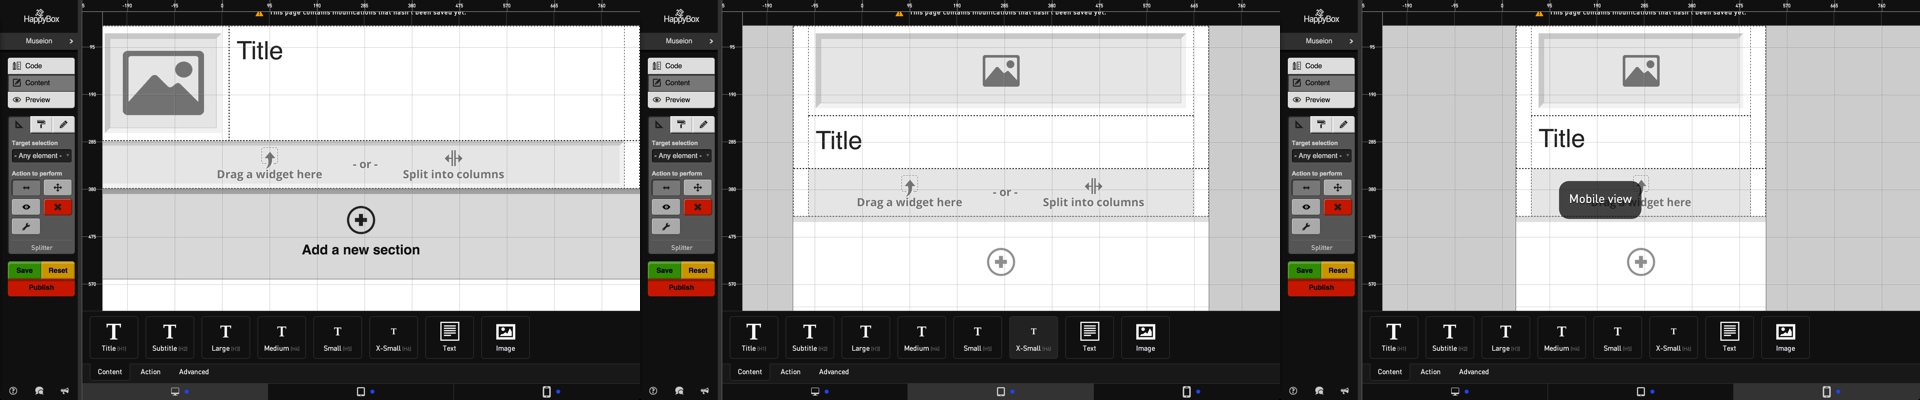
\includegraphics[width=\textwidth]{images/HBscreen/editeurGabarit.png}
		\caption{Editeur de Gabarit: vue ordinateur, vue tablette, vue mobile}

\end{center}

\paragraph{} % contenue, style, SEO
Une fois qu'une page est structuré il faut lui ajouter un style. Pour cela, un éditeur de style complet permettant de gérer la majorité des propriétées css via une interface simple d'utilisation permettant aux non-developeur d'affiner leur design avec un niveau de détails inégalé. Pour les utilisateurs confortable avec l'édition d'un fichier css, il possible d'écrire directement du code css dans l'éditeur.
Le contenue de la page, textes, images, sont éditable directement sur la page avec un rendu en temps réel. Ce que vous voyez c'est ce qui sera affiché.
Happybox garde en mémoire que la fonction premiére d'une page d'aterrissage est avant tout un outils de référencement vous permettant d'offir une meilleur visibilité à un produit ou un service pour le web. Un assistant de SEO est disponible dans l'éditeur proposant d'améliorer votre page en temps réel afin que les moteurs de recherche index au mieux la page.
%% screen contenue style CEO
\begin{center}
	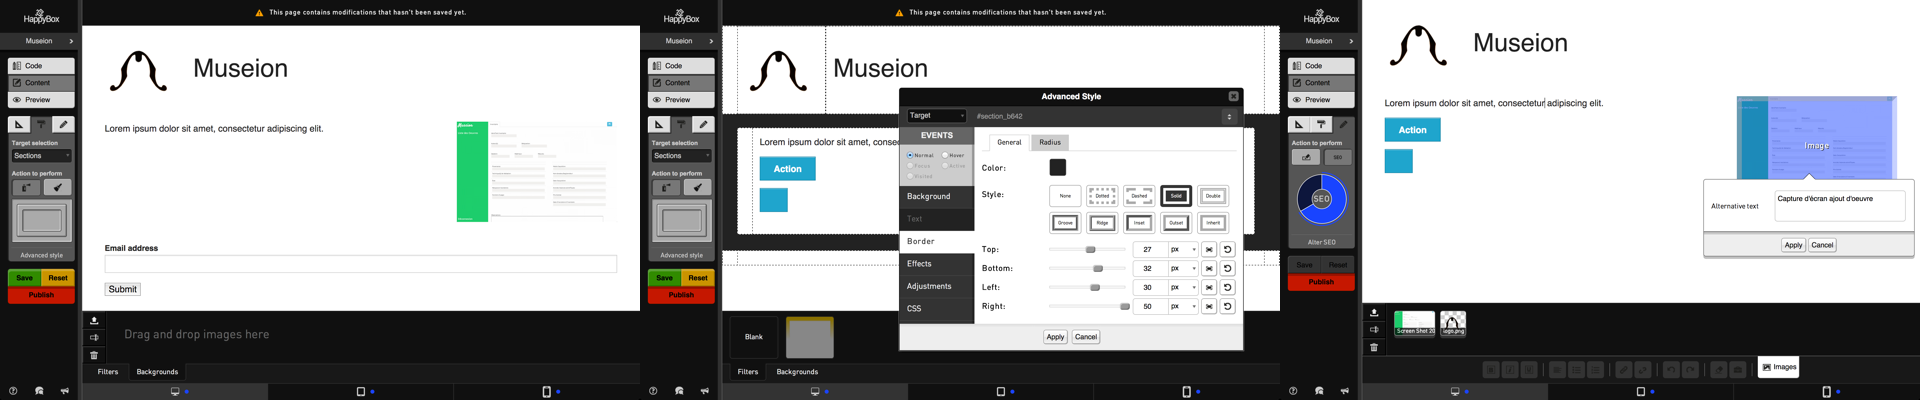
\includegraphics[width=\textwidth]{images/HBscreen/contenueStyleSeo.png}
	\caption{Editeur de contenue, editeur de style, editeur de SEO}
\end{center}

\paragraph{} % editeur de code + versionning
Happybox ciblant prioritairement les developeurs web, c'est pourquoi un éditeur de code permettant d'éditer l'intégralité des source de la page et d'ajouter des modules php ou javascript afin d'étendre encore les possibilités de la plateforme. Ce qui n'est pas déjà dévelopé par l'équipe pourra être dévellopé et tester avec un rendue en temps réel.
%% Screenshot editeur de source
\begin{center}
	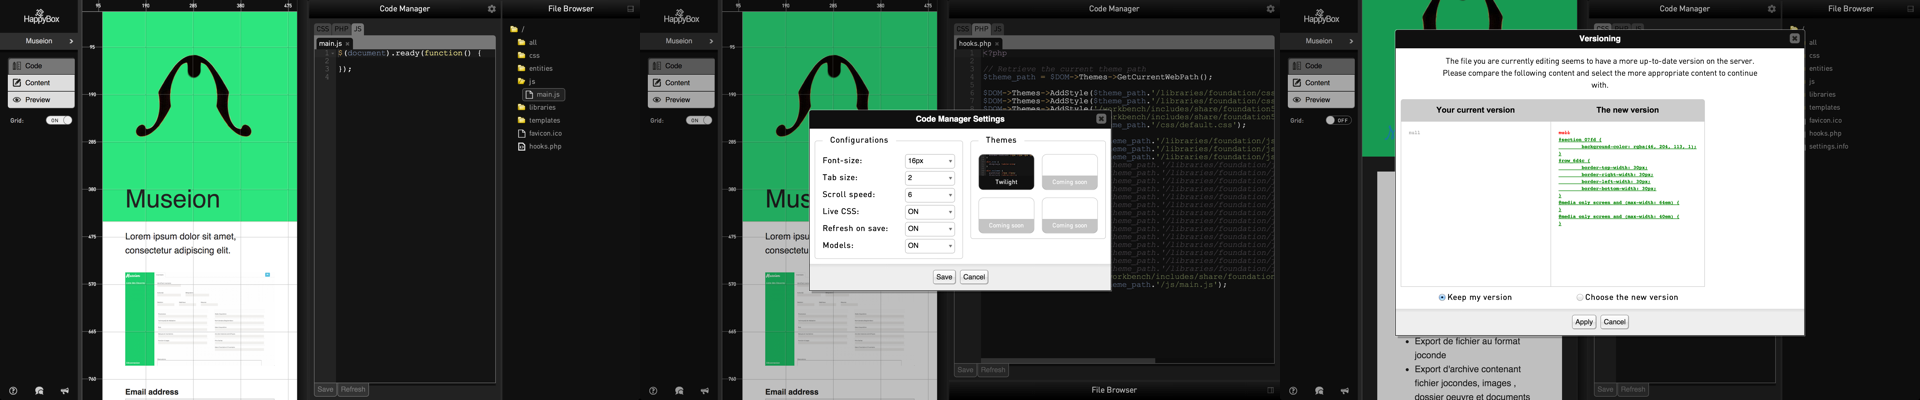
\includegraphics[width=\textwidth]{images/HBscreen/codeManager.png}
	\caption{Editeur de code: fichier php, configuration, gestion des versions}
\end{center}

% séparation fond et formes
\paragraph{}

Toutes ces fonctionnalité on pour finalité la création d'une page web unique. Il est donc possible de prévisualiser comme les utilisateurs le verront sur chaque type de résolution.
\begin{center}
	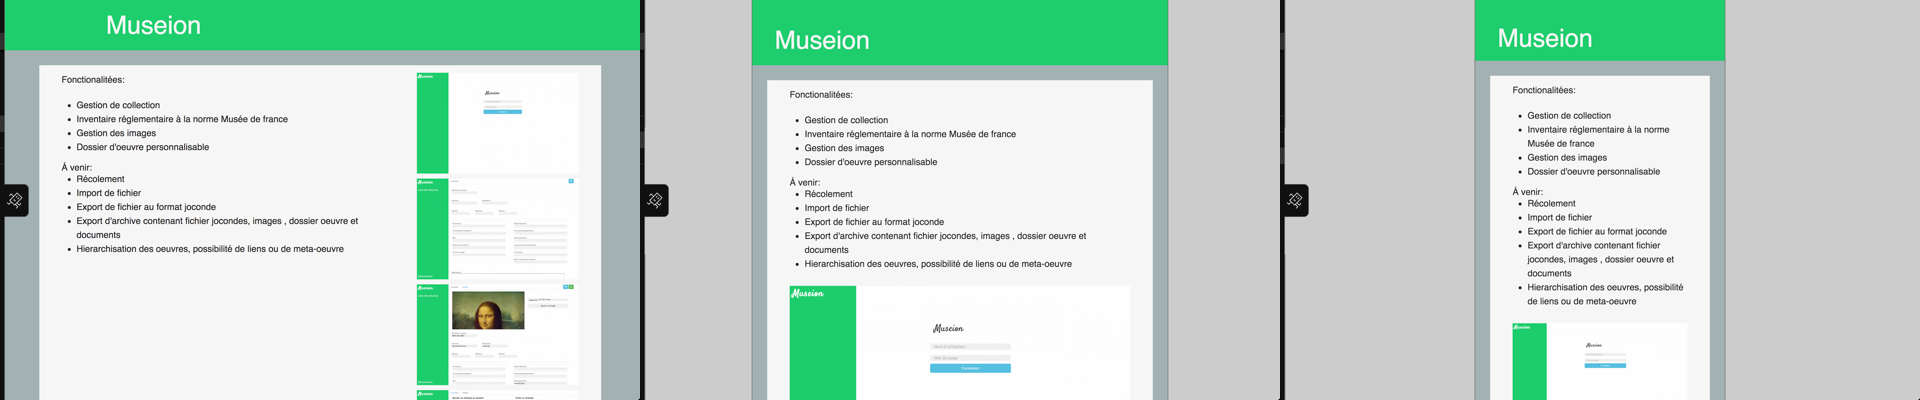
\includegraphics[width=\textwidth]{images/HBscreen/preview.png}
	\caption{Prévisualisation de la pages version ordinateur, tablette et mobile}
\end{center}

% présentation des outils de gestions
\paragraph{}
De plus chaque client ce vois allouer un espaces dédié sur nos serveurs. Il reste ainsi le seul et l'unqiue propriétaire de ses données. Happybox est donc aussi un hébergeur de données. Afin de répondre à cette seconde problématique un ensemble d'outils permettant d'accéder à ses statistique d'utilisation de stockage, la gestion des noms de domaines, d'analyser le traffique sur les pages.

\begin{center}
	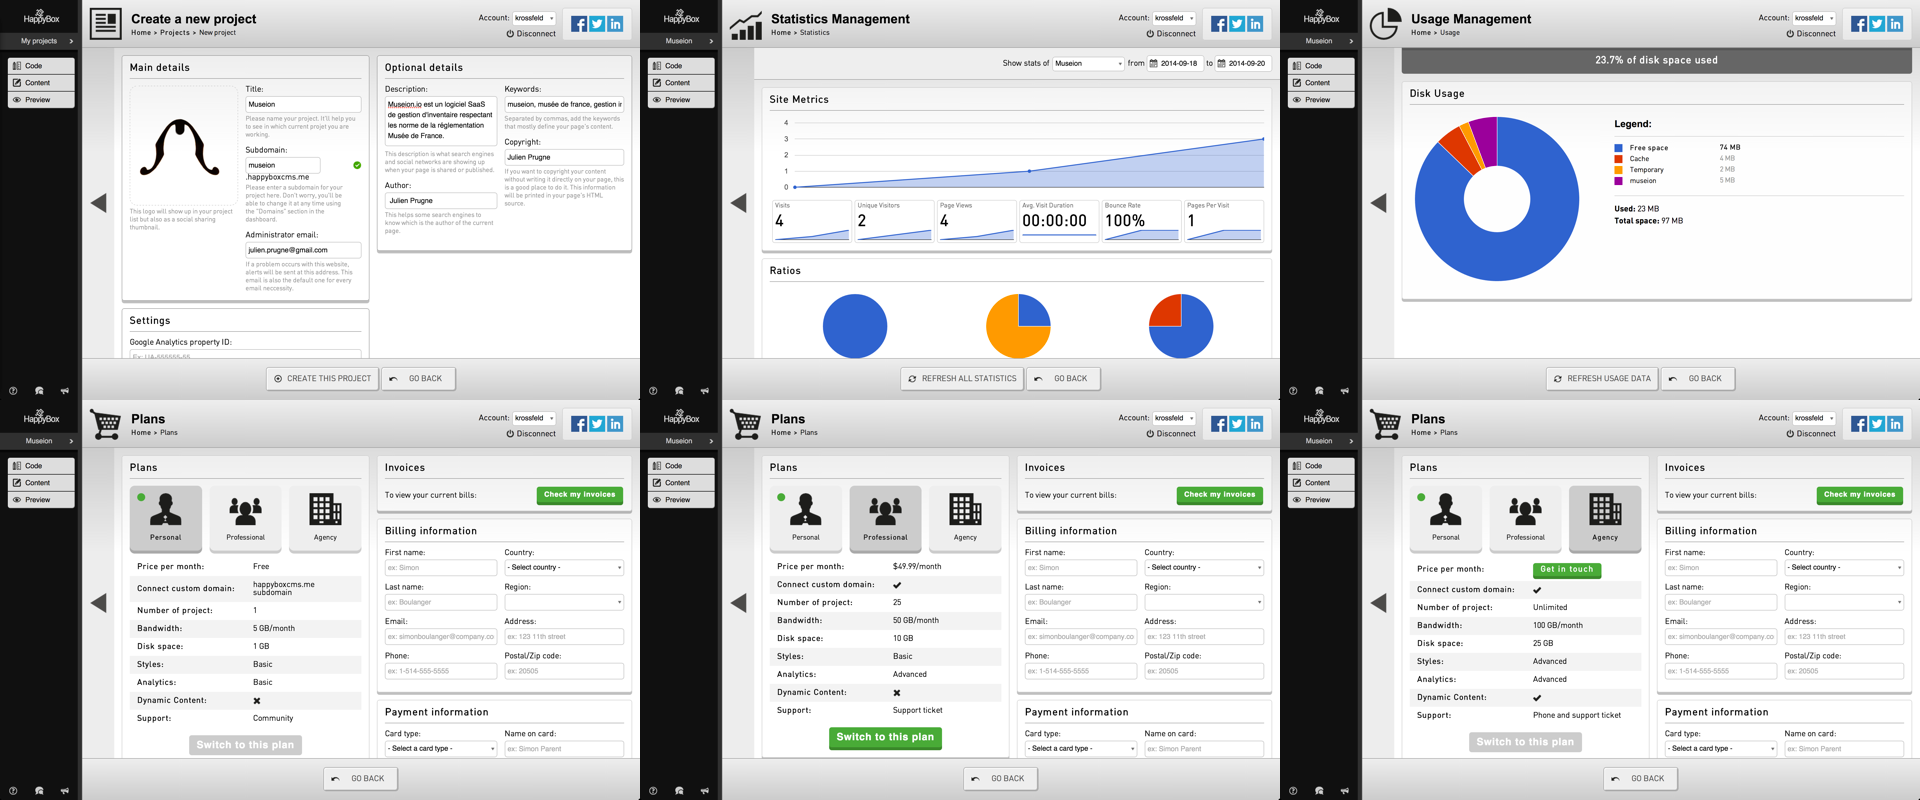
\includegraphics[width=\textwidth]{images/HBscreen/dash.png}
	\caption{Differentes options du panneau d'administration et différents forfait proposé}
\end{center}


	\subsection{Étude de l'écosystéme des startups}		

% http://blogs.wsj.com/accelerators/2013/06/24/steve-blank-the-6-types-of-startups-2/
		\paragraph{Présentation de 6 principaux\cite{typeStartup} types de startups}

			\subparagraph{Le style de vie startup:} %style de vie
Le premiers type de startupeur cherche le style des startups, il ne travail pour personne et vive de sa passion. Typiquement un surfer californien offrant des leçon de surf pour payer les factures et passer un peu plus de temps sur sa planche. Il ne s'agit pas réellement d'une startup dans le sens ou son objectif n'est pas de \emph{démarrer} et de connaitre une croissance rapide.

			\subparagraph{Les petites entreprises:} % petite entreprise
Les seconds sont des entrepeneurs opérant de petite entreprises, ils sont généralement boucher, coiffeurs, dévellopeur, et bien d'autre chose encore. Ils ont créer leur structure grace à leurs économies ou l'argent qu'ils ont pu emprunter. Ils ne correspondent pas non plus à l'image médiatique des entrepreneurs et leurs compagnie n'est pas adapatable à un marché de masse. Ils ne sont pas pour autant négligeable, en terme de statistique c'est le profile majoritaire des entrepreneurs.

			\subparagraph{Les mandatés par une plus grosse structure:} % filiale grosses entreprise permettant de tester de nouveaux modéles
De nos jours la pluspart des grosses entreprises ce sente menacé par ces nouveaux acteurs à croissance démentielle. Elles ont donc essayé de trouver une parade afin de garantir un flux continue d'innovation dans les méthodes d'affaire ainsi que dans le dévellopement de nouvelles technoliges. Les fondateurs sont mandaté par une entreprise afin d'externaliser un dévellopement afin de prendre un minimum de risque pour la filiale mère. Ces grosses entreprise possédant les fond nécessaire au dévellopement de sa filiale lui garantira une survie et un rachat si les objectifs sont atteint. Cette pratique permet de déroger aux pratiques manageriale et à la hierarchie souvent lourde, il est ainsi possible dévelloper le produit (bien de consomation, services, brevet(s), ...). Ce sont des laboratoire technoligque limitant les risques\footnote{En cas d'echec seuls les fonds investits sont perdu.}

			\subparagraph{Startups à vocation sociale} % à vocation sociale ex I can go without
Ce type de startup est unique, il ne cherche pas prioritairement à vendre un produit ou un services commerciale. Les fondateurs sont des idéaliste ayant un plan pour améliorer le monde ou essayer en tout cas.
Ils peux s'agir d'organisme à but non-lucratif, lucratif ou hybride alliant ainsi le meilleurs des deux monde.
En effet, une startup vivant principalement par ses flux entrant de capitaux entrant, il peut être nécessaire d'offir un modéle intégrant une perspective de rentabilité en plus de sa vocation phylantropique et un placement interessant en terme d'image pour l'investisseur ou le mécénes. Leurs sources de financement sont  multiples: dons, mécénats, venture capitalism, ange des affaires, financement participtif, subvention, ...
C'est un modéles particulièrement adapté à des missions humanitaires, des projets de dévellopements durables.


			\subparagraph{Les \emph{tout dois disparaitre}, créer pour être vendue} % Buyable ex: dev dúne techno puis vente trouver des exemples
Ces structures n'ont qu'un seul objectif: créer un produit pouvant être vendue le plus vite possible et le plus chères possible. Majoritairement les fondateurs de telles structures sont expérimenter et ont un domaine d'expertise poussé\footnote{Quel qu'en soit le domaine.} leurs permettant s d'analyser le marché et d'y trouver des niches d'innovations. Ces niches doivent être exploiter rapidement afin d'arriver avant que la concurrence ne ce soit créer. Proposant ainsi un produit ayant une valeurs ajouté importante car unique ou technologiquement supérieur à ses concurents. Une fois qu'ils ont vendue leur société pour une somme généralement comprise entre \$500,000 à \$50,000,000, ces derniers cherchent une nouvelles pétites d'innovation qu'ils pourront financer avec une partie de la vente de la compagnie précédente.

			\subparagraph{} %scalable % google, facebook, doyourfreemi
Finalement viennent les statups conçue dans leurs essences pour l'évolutivité. Ces compagnie visent généralement des taux de croissance extrémement rapide et nécessite de fond important permettant de soutenir leurs besoin de croissance, mais pas d'inquiétude des fond d'investissement géréer investisseurs appelé \emph{venture capitale\footnote{Capitalisme d'aventure}}. La majorité de ces startup mourrira avant de connaitre le destin glorieux et porteur de millionaire du mythe de la startup. Facebook, google, twitter sont des exemples de stratup ayant basé leurs ayant basé leur stratégie sur l'adaptabilité et l'évolutivité sont devenue des méga-corporations internationale ne se limitant plus à leurs domaine d'origine.

		\paragraph{La chaine d'approvisionements }
	
L'économie traditionnel peux être définie par sa chaine de distribution des biens, dans ce modéles un \emph{fournisseur/créateur} vend sa production à une \{plateforme de centralisation des biens} qui ce chargera ensuite de les distribuer et de les vendres au consommateur. Le concept est simple acheter à moindre pour ensuite revendre à un prix supérieur ceci permettant de dégager une \emph{recette} qui dois être supérieur à la somme coût. Si la recette est supérieur aux coûts alors l'opération génére des bénéfices qui peuvent être réutiliser dans l'entreprise créant ainsi un cercle vertueux d'investissement.

D'autre modéles d'approvisionnement propose d'offrir un service gratuit aux consommateurs tout en achetant les biens qui leurs sont distribué.
L'injection de publicité dans le services permettra de monétiser le ce dernier. Mais méfiance car ceci n'est possible que si beaucoup d'utilisateurs utilise le produit gratuits. En effet ce n'est pas la publicité en elle même qui représente une valeur ajouter mais sa diffusion devant un publique aussi important que possible. C'est la méthode fonctionnement des journaux gratuits, de certaine chaine de télévision, de Youtube par exemples. La seul réelle condition d'un tels modéles est dávoir une large base d'utilisateurs permettant de valoriser la diffusion de la publicité.

L'industrie du disque par exemples à adopter un modéle bi-directionnel. Ce qui signifie qu'un musiciens \emph{doit} payer une maisons de disques par l'intermediaire de commission\emph{Et plus insidieusement par la perte de ses droits sur son travail car l'artiste ne posséde que le droit d'en être l'auteur mais la maisons de disque possèdent les droits sur les enregistrements.} pour qu'elle enregistre, et distribue auprés des consommateurs afin que ces derniers est l'opportunité d'acheter. C'est un modéle qui ne favorise que l'acteur centrale qui touche des recettes à la fois de ses clients et de ses fournisseurs.

La proposition de chaine d'approvisionnement par les utilisateurs, peut être exploré mais ce modéles compte sur l'autonomie des utilisateurs à s'amuser les uns avec les autres. Les utilisateurs crée et consomme le contenue, le tout gratuitement et pour toujours. C'est à mon goût une vision naïve car il est impossible de maintenir un niveau de qualité permettant d'attirer de nouveaux utilisateurs. De bon exemples du modéles UGC sur les plateformes web serait tumblr qui propose un service de blogging communautaire gratuit mais la majorité des plateformes UGC ressemblent plus au site \emph{4chan} et ce n'est pas particuliérement jolie à voire.

Tout ces modéles de gestion sont intéressants. Ils offrent chacun leur avantages et leurs inconvenients mais ils ne peuvent répondrent au besoin de croissance d'une entreprise adoptant le modéles freemium.

Une chaine de distribution différente c'est alors créer autour de l'écosystéme de ces entreprises à forte croissance et au potentiel énorme. Plusieurs niveaux de financement sont accessible aux entreprises présentant de forte chance de rentabiliser l'investissement rapidement. Les startup on certe un énorme taux d'echec mais en cas de revente elle représente un taux de retour sur investissement suffisant à compenser les pertes dues aux échecs.

		\paragraph{Aparte sur financement des startup}
Il deux grand type de recoltes de fond pour une startup: les subventions directe et les subevention indirectes. 
Les subventions directes sont obtenues via des bourses, lors de la participation à des concours entrepreunarial

%%%% FINACEMENT HB %%%%%
%Avril 2013 Fondation Montréal Inc. (12 000)
%Juin 2013 Jeunes Promoteurs (18 000)
%Février 2014 SDEVM (10 000)

%%%%%%%%%%%%%%%%%%%%%%%%%
		\paragraph{Critique}
		% VC et angel fournisseur d'un bien précieux du pognon
		% une startup meurt ou multiplie les capitaux
		% explosion bulle spéculative 29, bulle internet, Sub primes
			% actif en circulation ne represente pas la valeur réel =>
		% critique du modéles


		\subsection{Secteur à forte concurrence}

Le monde des gestionnaire de contenue est un secteur à




	%\chapter{Problématique} % 28 pages
		\section{problématique} % 5 pages

% de gagner en perfomance, en disponibilités, de simplifier les taches d'administration en faisant abstraction de la couche matérielle.


Il est de plus en plus courant de recourir au service de cloud\footnote{appelé aussi informatique en nuage} public afin de proposer une infrastructures évolutive capables de répondre à une croissance rapide de la base d'utilisateurs et de s'adapter en conséquences.
Malgrès leurs apparences attirantes\footnote{trés haute disponibilité, flexibilité, sécurité, faible coût annoncé ...} les plateformes dites IaaS, Infrastructure as a Service\footnote{Infrastructure comme un Service}, engendre un lot de coût  caché et de nouveaux défis dans la gestion des systèmes d'information.


 Il semble donc nécessaire de mettre en place une politique de gouvernance afin de réellement exploiter le potentiel de telles infrastructures pour achever un taux de croissance important, un cout par utilisateurs minimale et une capacité d'adaptation optimale. Comment et par le biais de quels indicateurs pouvons atteindre cet objectif.


			%Explication et developement de la problématique
			\subsection*{}
				%terminologie
				%\subsubsection*{}

Avant d'aborder le vif du sujet il me semble nécessaire d'expliciter un certain nombre de termes et concepts qui sont utilisés dans la problématique et s'avèrent fondamentals à la compréhension de ce document.
					%cloud
					%\paragraph{}
						%definition Cloud computing en géneral

Le cloud computing\cite{cloudDef}\index{Cloud computing!Définition} est une pratique visant à dématérialiser les infrastructures des services d'information. Elle entraine un changement fondamental dans le paradigme d'accès aux ressources informatiques. En effet, les machines hôtes ne sont plus accessibles physiquement mais virtualisées à l'aide d'un hyperviseur\index{Hyperviseurs}.

Les hyperviseurs sont des plateformes de virtualisation permettant d'éxécuter plusieurs systémes d'exploitation dit invités\index{systéme invité} sur une même machine dite hôte\index{systéme hôte} ou une ferme de calcul\footnote{Appelé également grappe de serveurs ou encore cluster. Il s'agit d'un ensemble d'ordinateurs reliés les uns aux autres, mettant leurs ressources en commun, créant ainsi une sorte de \emph{super ordinateur}. }.

Cela crée ainsi une abstraction entre la gestion physique du matériel et l'exploitation des ressources informatiques. Ainsi, la mise en place d'un serveur ne se fera plus en achetant et en installant un nouvel hôte dans son centre de données, mais via la réservation et la création de machines virtuelles.

Un hôte physique hébergera donc un ou plusieurs systèmes d'exploitation et l'hyperviseur se chargera d'allouer ou non les ressources\footnote{unité de calcul, mémoire, stockage, accès réseaux, ...}  physiques nécessaires via des interfaces virtuelles accessibles depuis la machine virtuelle comme si ces derniers étaient physiques. Le système invité ce comportera comme si il possédait son propre matériel.

Les nuages peuvent être classés dans deux catégories: les cloud privés et les cloud publiques.

						% définition cloud privé

Les cloud privés\index{cloud privé|nuage privé! définition} sont des infrastructures physiques\footnote{serveur isolé ou en grappe} loués ou hébergés dans un centre de données et uniquement utilisés par le locataire ou propriétaire. Ils sont physiquement accessibles par les administrateurs qui seront responsables de leur bon fonctionnement. Si les ressources fournies par le nuage privé viennent à manquer, il sera du ressort des exploitants\footnote{propriétaire ou locataire des infrastructures} d'acheter, de configurer et d'installer un nouvel hôte dans la ferme de calcul afin d'augmenter les ressources allouables aux systémes invités. Á puissance égale ces infrastructures semblent moins dispendieuses que les cloud publiques mais les moyens humains nécessaires à la mise en place et la maintenance de telles solutions sont conséquents.

						% définition cloud public
Les seconds, dis nuage public\index{cloud public|nuage public! définition}, sont des infrastructures accessibles généralement via des applications web et/ou des interfaces de programmation\footnote{API: Application Programming Interface}. Les ressources sont accessibles en libre service et à la demande. Le prestataire facturera à l'utilisation\footnote{Exemple: volume de données hébergées, mémoire utilisée par une application, bande passante, ...} ou de manière forfaitaire\footnote{Location annuelle d'une instance, réservation d'un espace de stockage dédié, ...}.

					%\paragraph{IaaS/PaaS/SaaS} transition TODO:definir serrvice web
					%utiliser pizza as a service comme exemple
				% résumé
Les clouds publiques sont generalement composés de trois types de services\index{service|service web!définition}\footnote{Un service web\cite{webServicesDef} peut être défini comme étant une interface logicielle permettant un accès standardisé à un ensemble de ressources hétérogènes via internet ou un réseau intranet.}:
\begin{description}

	\item[IaaS\index{IaaS|Infrastructure as a Service}, Infrastructure as a Service, Infrastructure comme un Service] Amazon Web Services, Google Compute Engine, Digital Ocean

	\item[PaaS, Plateform as a Service, Plateforme comme un Service] Heroku, Google App Engine, dotCloud, Amazon Opswork

	\item[SaaS, Software as a Service, Logiciel comme un Service]
	Happybox CMS, Gmail, Jira, Museion

\end{description}

Pour bien expliquer ces différents concepts, nous nous réfererons à l'excellente analogie \emph{Pizza comme un Service}\cite{PizzaasaService}. Cette dernière nous explique que les habitudes d'utilisation de plateforme en ligne sont comparables aux habitudes de consommation de pizza.

En effet, un cloud privé\index{Cloud privé!Définition par la pizza} où vous vous chargeriez d'équiper les locaux en éléctricité, en ventilation, de gérer la sécurité physique et logicielle et installer les serveurs dans votre centre de données serait comparable à faire votre pâte à pizza, garnir votre pizza, la cuire, installer votre table à manger, servir les boissons et votre pizza. Cette solution vous offre le plus de fléxibilité dans les choix que vous pouvez faire mais peut devenir très contraignante car tout est de votre responsabilité.

Les solutions IAAS\index{IaaS!Définition par la pizza}, sont comparables au fait d'acheter une pizza crue ou congelée et de la cuire chez vous. En d'autres termes vos considérations s'orienteront sur le choix et l'installation des sytémes d'exploitations, la création de réseaux virtuels, la configuration de gestionnaire de charge\footnote{load-balancer}... Ces services vous offrent un centre de données complet sans les inconvénients du matériel.

Les solutions PaaS\index{Paas!Définition par la pizza} correspondent au service de livraisons de pizza. Il ne reste à votre charge que la table et les boissons. D'un point de vue informatique, vous géreriez la création de votre application puis la déploierez chez votre fournisseur. La gestion du systéme d'exploitation n'est plus de votre ressort vous laissant la responsabilité de votre logiciel.

Finalement les solutions SaaS\index{SaaS!Définition par la pizza} sont le pendant logiciel des pizzerias. Il vous suffit de payer, ou de laisser la plateforme collecter vos informations personelles en guise de paiement, pour accéder aux services et rien n'est de votre ressort à part votre utilisation. Il s'agit d'une évolution de la livraison et de la consommation logicielle.

Le schéma ci dessous illustre ces explications:

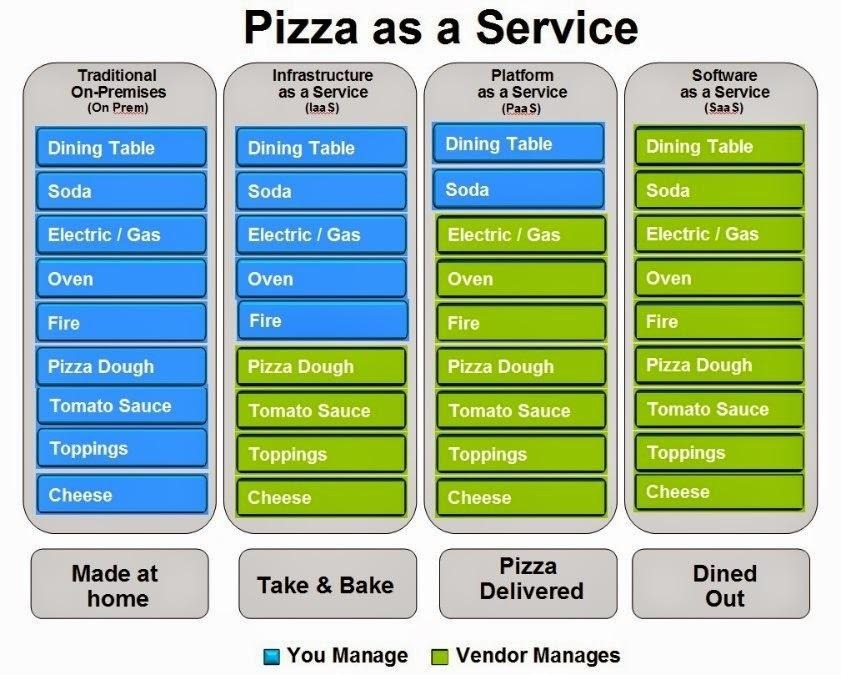
\includegraphics[width=\textwidth]{images/PizzaasaService.jpg}

				%\subsection*{approche envisagé}

					%\paragraph{cout}
					%\paragraph{consitence de la conf}
					%\paragraph{sécurité et privacité}
La frontière entre ces différents types d'infrastructure est parfois mince voire inexistante. Par expemle, la plateforme web permettant de gérer ses infrastructures virtuelles chez n'importe quel fournisseur d'infrastructure comme un service\footnote{IaaS} n'est autre qu'un logiciel comme un service\footnote{SaaS}. De plus, les plateformes IaaS fournissent généralement une solution de plateforme comme une service\footnote{PaaS}. Google app Engine est une plateforme PaaS fournis par google et inclus dans l'offre Google Cloud, de la même façon Amazon Web Service propose Opswork.

De fait, ces concepts restent trés théoriques et leurs implémentations ne sont jamais une vision absolue du concept. Il est donc important de bien comprendre ces services afin de définir le potentiel de chaque plateforme d'hébergement et d'en exploiter au maximum les fonctionnalitées.
Pour cela, nous utiliserons sept d'indicateurs permettant, selon mon expérience, de comparer la pertinence des différentes solutions présente sur le marché.

\begin{description}

	\item[Sécurité]
		Controller l'accès aux ressources et aux données. Pouvoir garantir leur confidentialité.

	\item[Souveraineté]
		Posséder totalement ou partiellement ses ressources et données.

	\item[Flexibilité]
		Changer, ce transformer, s'adapter aux besoins des utilisateurs.

	\item[Consistence]
		Garantir la configuration, les mises à jours.

	\item[Cout]
		Le nerf de la guerre qu'il faut savoir gérer pour ne pas ce retrouver sans éléctricité pour ses serveurs.

	\item[Compétence nécessaire]
		Besoin en formation ou en personnel qualifié.

\end{description}

Ces indicateurs, devrait à eux seuls permettre de définir notre politique de gouvernances. Ils sont, en quelques, sorte les indicateurs vitaux d'un systéme informatique.

		% Méthodes habituellement utilisé pour une situation présentant des similitude
		\section{méthodes habituelles} % 5 pages

1 sys admin = X serveurs
1 sysadmin = 1 corps
1 corps peut physiquement y serveurs

X tant à augmenter mais pas le nombre de corps/sysadmin => ratio merdique de 1


			\subsection{Création de centre de données et cloud privé}
\paragraph{Présentation}

\paragraph{Points forts}

\paragraph{Points faibles}

\paragraph{Conclusion}

			\subsection{Déploiement manuel ou scripté}

		% Exposé des décisions prise et des interventions menée par le stagiare pour résoudre le problème
		\section{Une infrastructure à batis dans le nuage.}	 % 15 pages

			\subsection{Déploiement happybox CMS}
				% montrer que ça demande beaucoup de temps et d'efforts
				% peu de moyen et peu de monde
			\subsection{AWS}
				% analyse des coups, explication IAAS
				% présentation argumenté de AWS/GCE

			\subsection{Opswork}
				% gestion configuration, automatisation déploiement, productivité

			\subsection{Open source: Gitlab, Open Web Analytics}
				% impact du logiciel libre sur le travail
				% Ouverture sur le possible future libre de Happybox CMS

		% Démonstration d’une originalité dans l’élaboration et la mise en œuvre de la solution
		\section{Demonstration que c'est trop plus la bonne décision} % 5 page
				% gain productivité
				% gain cout
				% gain maintenabilité
				% gain scalabilité
				 % gain sécurité

		% Analyse de l’approche choisie
		\section{Analyse masturbatoire de l'action} % 3 pages
				% c'est le moment de ce la péter

		% Réflexion sur le stage et le mémoire
		\section{Autoévaluation}

	\section{Conculsion} % 2 pages

	\section{Remerciements}

	\appendix
	\section{Exemples de pages Happybox}

	\section{Plan freemium}
	%bibliographie
	\printindex

	\bibliographystyle{amsplain}
	\bibliography{bibli}
\end{spacing}
\end{document}
